%    DO NOT CHANGE THE SETTINGS BELOW
%%%%%%%%%%%%%%%%%%%%%%%%%%%%%%%%%%%%%%%%
\documentclass[12pt]{article}
\usepackage{epsfig}
\usepackage{graphicx,float}
\usepackage{url}
\usepackage[hidelinks,colorlinks=true,bookmarks=true]{hyperref}
%*******************************************
\setlength{\textheight}{24cm}		
\setlength{\textwidth}{17.5cm}		
\setlength{\oddsidemargin}{-0.5cm}
\setlength{\topmargin}{-1.25cm}
%*******************************************
\pagestyle{empty} 

% \usepackage{graphicx}
% \usepackage{caption}
\usepackage{subcaption}
\newtheorem{theorem}{Theorem}
 
\def\gcg{\mathcal{G}}  % Granger-causality graph
 
\begin{document}
\hspace{-0.70cm}\rule{17.5cm}{0.01 in} \\
\vspace{-0.4cm}
\begin{flushleft}
  \Large \textbf{\noindent Graph Topological Aspects of Granger
    Causality in Stationary Linear Dynamical Systems}
%%%%%%%%%%%%%%%%%%%%%%%%%%%%%%%%%%%%%%%%%%%%%%%%%%%%%%%%
\\
%%%%%%%%%%%%%%%%%%%%%%%%%%%%%%%%%%%%%%%%%%%%%%%%%%%%%%%%
\vspace{0.5cm}
\normalsize
 %%%%%%             NAMES OF AUTHORS         %%%%%%
 %%%%%% NAME OF SPEAKER SHOULD BE UNDERLINED %%%%%%%%%
\normalsize{
 \underline{Ryan J. Kinnear}$^1$, Ravi R. Mazumdar$^1$
} \\
\vspace{5mm}
\textit{\footnotesize
 %%%%%% AFFILIATION OF AUTHORS %%%%%%
$^1$ Department of Electrical and Computer Engineering, University of Waterloo, Waterloo, Ontario N2L 3G1, Canada\\
 %%%%%%%%%%%%%%%%%%%%%%%%%%%%%%%%%%%%%
}
\end{flushleft}

The concept of Granger causality, a notion introduced in 1969
\cite{granger1969investigating} for the analysis of macroeconomic data
(e.g. ``does lowering the interest rate cause an increase in
employment?''), attempts to capture the intuition that a cause must
proceed it's effect, and has spurred both theoretical and applied
research.  The concept has been applied in diverse settings, for
example: in finance, researchers have attempted to quantify the
interdependence of financial institutions \cite{NBERw16223} and in the
biological sciences, the concept is used to map out the promoting and
regulating effects of certain genes upon others
\cite{methods_for_inferring_gene_regulatory_networks_from_time_series_expression_data}.

A substantial portion of the work on this topic is devoted to
generalizing the methods of Granger to nonlinear systems.  For
example, linear Granger causality is a special case of the information
theoretic notion of transfer entropy \cite{barnett2009granger}.
However, like many attempts at quantifying causation, transfer entropy
suffers from some difficulties of interpretation
\cite{transfer_entropy_criticism}.  Although the criticisms raised by
\cite{transfer_entropy_criticism} do not arise in the case of linear
Granger causality, other pathologies are known.  Our work sheds light
on some of the challenges that remain in the linear case, and in
particular focuses on topological particularities of the underlying
network of interactions.

In general, we are presented with a multitude of jointly wide sense
stationary time series $x_1(t), \ldots, x_n(t)$ and seek to construct
a (Granger-)causal graph $\gcg$ where there is an edge
$(j, i) \in \gcg$ whenever $x_j$ Granger causes $x_i$ after
conditioning on each $k \not\in \{i, j\}$.  Depending on the
interpretation or on the application, the graph $\gcg$ captures the
flows of ``information'' or ``energy'' throughout a network of
interacting processes.  However, it may be the case that we observe
$x_j$ and $x_i$ alone -- in such cases, simple examples establish that
even if $x_j$ Granger causes $x_i$ conditioned on the rest of the
observations, it need not be that $x_j$ Granger causes $x_i$ pairwise
(i.e. without conditioning).

Pathologies of pairwise causation clash with our intuition that causal
relations in $\gcg$ should be transitive, that is, that if there is
some ``true'' (conditional) causation path
$j \rightarrow a_0 \rightarrow \cdots \rightarrow a_r \rightarrow i$
in $\gcg$ then it should hold that $x_j$ pairwise causes $x_i$.  While
this does not hold in general, our work analyzes a particular type of
graph topology, which we deem a ``strongly causal'' graph, wherein
natural intuitions about causal flow \textit{do} hold.  Moreover, we
prove that (with modest additional technical assumptions) that in such
a graph the complete conditional causation graph $\gcg$ can be
recovered by testing only pairwise interactions of nodes.  That is,
the complete causal structure of $\gcg$ can be recovered through
simple one way unconditional causality tests.

The flavour of this work may be conveyed by stating one of our main
conclusions, where the ideas behind $T_{ij}(z)$ are subtle and not
expanded upon in this brief summary.

\begin{theorem}[Pairwise Recovery]
  \label{thm:scg_recovery}
  If the Granger causality graph $\gcg$ for the process $x(t)$ is
  a strongly causal DAG and $T_{ij}(z)$ is a two-sided filter for every
  $i, j \in [n]$, then $\gcg$ can be recovered from pairwise causality
  tests alone.
\end{theorem}

% \begin{figure}[h]
%   \centering
%   \begin{subfigure}[b]{0.45\textwidth}
%     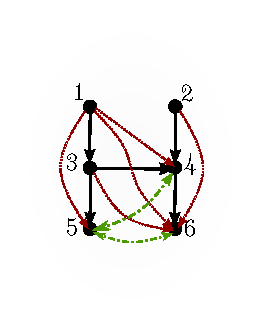
\includegraphics[width=\linewidth]{../../figures/example_algorithm.pdf}
%   \end{subfigure}
%   \begin{subfigure}[b]{0.45\textwidth}
%     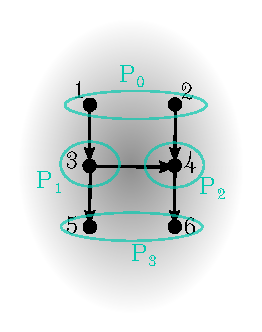
\includegraphics[width=\linewidth]{../../figures/example_algorithm2.pdf}
%   \end{subfigure}
% \end{figure}

\begin{figure}[h]
  \centering
  \caption{Recovering Large Networks via Pairwise Causality Tests}
  \label{fig:large_n_figure}
  \includegraphics[width=0.7\linewidth]{../../figures/new_increasing_n_simulation.pdf}
\end{figure}

Our concept of a strongly causal graph topology initially arose
artificially as a technical condition to understand the intuition of
causality flow in $\gcg$ and to establish Theorem
\ref{thm:scg_recovery}.  However, examples from the gene regulatory
network literature suggest that the dynamics of some natural
interacting systems may have an underlying interaction graph which is
in fact strongly causal, or at least nearly so.  Simulation evidence
also suggests that our algorithm for graph recovery via pairwise
testing can outperform the widely employed LASSO (and variations
thereon) for systems which satisfy (or nearly satisfy) the strongly
causal condition; in the process we make the incidental observation
that, all else equal, the LASSO exhibits superior performance on the
strongly causal topology than on a general directed acyclic graph,
suggesting that topological aspects of the underlying causality graph
may be of interest as an aspect unique to time series data in
comparison to ordinary regression.  Finally, the results of Figure
\ref{fig:large_n_figure} show that when topological assumptions are
met, it is possible to accurately identify extremely large networks
($n > 1000$, implying more than $10^6$ possible edges), and that the
underlying graph topology is an important determination of estimation
accuracy in addition to the simple size and sparsity of the network.
 
 % Please send your source file  and .pdf file to Alyssa Novelia (anovelia@uwaterloo.ca) or Isam Al-Darabsah (ialdarabsah@uwaterloo.ca)

%%%%%%%%%%%%%%%%%%%%%%%%%%%%%%%%%%%%%%%%
%% BIBLIOGRAPHY
%%%%%%%%%%%%%%%%%%%%%%%%%%%%%%%%%%%%%%%%
\begin{thebibliography}{00}
\addcontentsline{toc}{chapter}{References}
\setlength{\itemsep}{-1mm}
\small
\bibitem{granger1969investigating} Granger,
  C. W. J. (1969). \textit{Investigating causal relations by
    econometric models and cross-spectral methods.} Econometrica 37
  (3), 424–438.

\bibitem{NBERw16223} Billio, M., M. Getmansky, A. W. Lo, and
  L. Pelizzon (2010, July). \textit{Econometric measures of systemic
    risk in the finance and insurance sectors.}  Working Paper 16223,
  National Bureau of Economic Research.

\bibitem{methods_for_inferring_gene_regulatory_networks_from_time_series_expression_data}
  Nguyen, P. (2019). \textit{Methods for Inferring Gene Regulatory
    Networks from Time Series Expression Data.}
  Ph. D. thesis, Northwestern University

\bibitem{barnett2009granger} Barnett, L., A. B. Barrett, and
  A. K. Seth (2009). \textit{Granger causality and transfer entropy
    are equivalent for gaussian variables.} Physical review letters
  103(23), 238701.
  
\bibitem{transfer_entropy_criticism} Ryan G James, Nix Barnett, and
  James P Crutchfield. \textit{Information flows? A critique of
    transfer entropies}. In: Physical review letters 116.23 (2016),
  p. 238701
\end{thebibliography}
\normalsize
\end{document} 
